\documentclass{IEEEtran}
\usepackage[utf8]{inputenc}
\usepackage[alsoload=synchem,load=named]{siunitx}
\usepackage[version=4]{mhchem}
\usepackage{amsmath}
\usepackage{graphicx}

\graphicspath{{images/}}

\let\DeclareUSUnit\DeclareSIUnit
\let\US\SI
\DeclareUSUnit\foot{ft}
\DeclareUSUnit\inch{in}

\author{Powers-Luhn, J.R.}
\title{Analysis of the Impact of Learning Rate and Time Dependence on a Linear Neural Network}
\date{June 13th, 2017}

\begin{document}
\maketitle

\section{Introduction}
An investigation was conducted into the ability of a single-layer neural network to model a linear equation.

\section{Methods}
\subsection{Training Rate}
A MATLAB script was written to iteratively train a neural network. The network had an input layer of two neurons, $x_1$ and $x_2$, a bias neuron, and a single output neuron. The network was trained with labeled data (as appropriate for a regression problem). One hundred input vectors (of two values each) were generated in the range $[0,1]$ using the MATLAB \verb|rand| command with a seed of 10. Output values were set to $ y=2x_1 - 3x_2 -1 $. The network was trained for 100 epochs, with error and weights recorded after each epoch. The learning rate was varied from $0.1$ to $0.9$.

\subsection{Time Dependence}
In order to test the impact of a time-dependent factor on the training, a loop was added to the code and the network output was trainined to match the function $ y=2x_1 - 3x_2 -1 + 0.02i $ with $i$ varying from 1 to 100 in steps of 1. The same learning rates were applied as in the Training Rate section above. As before, the value of the weights, bias, and error were recorded at each iteration.

\section{Results}
\subsection{Training Rate}
It was expected that the weights should converge on the coefficients of the input terms $x_1$ and $x_2$. In the cases where the learning rate was low (see figs \ref{fig:err01notime}, \ref{fig:wgt01notime}, \ref{fig:err03notime}, \ref{fig:wgt03notime})

\begin{centering}
\begin{figure}
\begin{center}
	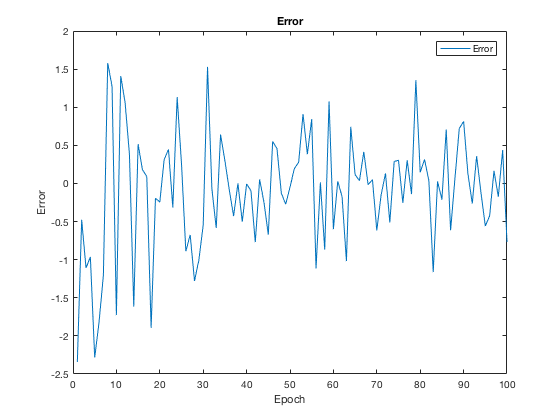
\includegraphics[width=0.4\textwidth]{error_notime_01lr}
	\caption{Error for each training epoch, learning rate = 0.1\label{fig:err01notime}}
\end{center}
\end{figure}
\end{centering}

\begin{centering}
\begin{figure}
\begin{center}
	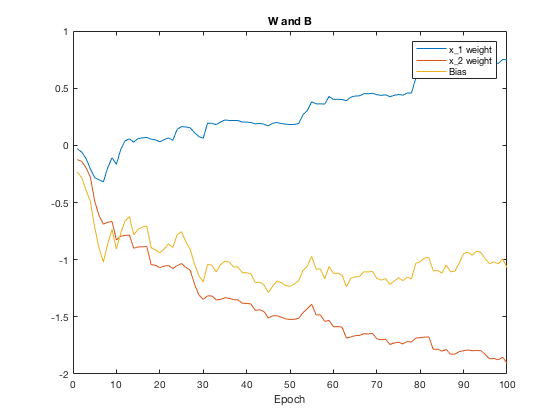
\includegraphics[width=0.4\textwidth]{weights_notime_01lr}
	\caption{Weights for each training epoch, learning rate = 0.1\label{fig:wgt01notime}}
\end{center}
\end{figure}
\end{centering}

\begin{centering}
\begin{figure}
\begin{center}
	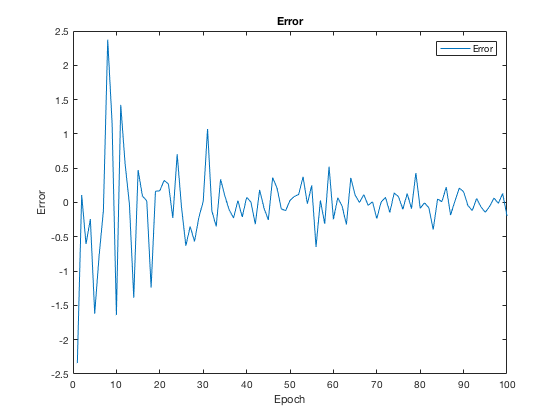
\includegraphics[width=0.4\textwidth]{error_notime_03lr}
	\caption{Error for each training epoch, learning rate = 0.3\label{fig:err03notime}}
\end{center}
\end{figure}
\end{centering}

\begin{centering}
\begin{figure}
\begin{center}
	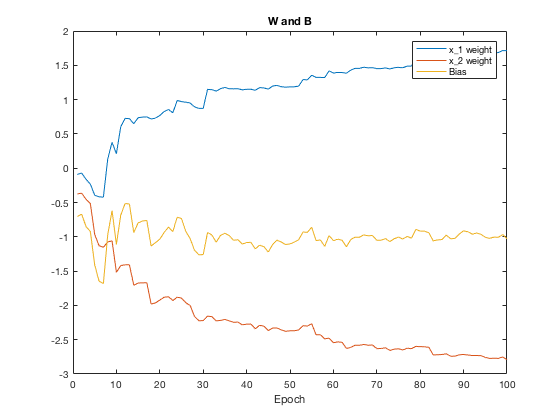
\includegraphics[width=0.4\textwidth]{weights_notime_03lr}
	\caption{Weights for each training epoch, learning rate = 0.3\label{fig:wgt03notime}}
\end{center}
\end{figure}
\end{centering}

With higher learning rates in place, the weights converged as expected (see figs \ref{fig:err07notime}, \ref{fig:wgt07notime}, \ref{fig:err09notime}, \ref{fig:wgt09notime}). It was theorized that the weights would have converged even with slower learning rates had more training epochs been run.

\begin{centering}
\begin{figure}
\begin{center}
	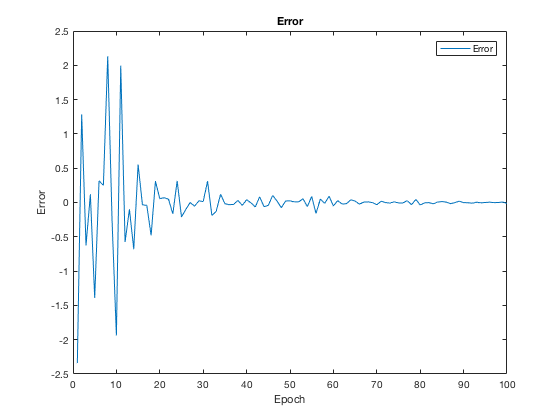
\includegraphics[width=0.4\textwidth]{error_notime_07lr}
	\caption{Error for each training epoch, learning rate = 0.7\label{fig:err07notime}}
\end{center}
\end{figure}
\end{centering}

\begin{centering}
\begin{figure}
\begin{center}
	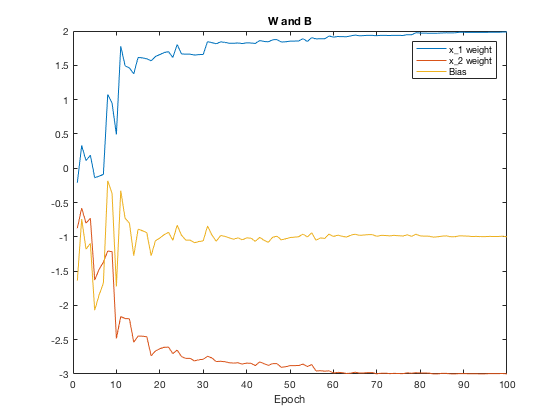
\includegraphics[width=0.4\textwidth]{weights_notime_07lr}
	\caption{Weights for each training epoch, learning rate = 0.7\label{fig:wgt07notime}}
\end{center}
\end{figure}
\end{centering}

\begin{centering}
\begin{figure}
\begin{center}
	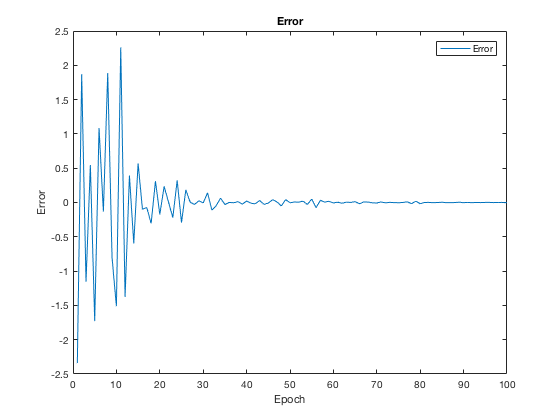
\includegraphics[width=0.4\textwidth]{error_notime_09lr}
	\caption{Error for each training epoch, learning rate = 0.9\label{fig:err09notime}}
\end{center}
\end{figure}
\end{centering}

\begin{centering}
\begin{figure}
\begin{center}
	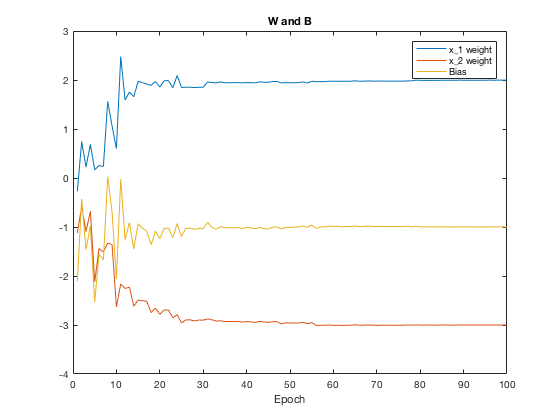
\includegraphics[width=0.4\textwidth]{weights_notime_09lr}
	\caption{Weights for each training epoch, learning rate = 0.9\label{fig:wgt09notime}}
\end{center}
\end{figure}
\end{centering}

\subsection{Time Dependence}
The introduction of a time dependent factor (see figs \ref{fig:err01time}, \ref{fig:wgt01time}, \ref{fig:err03time}, \ref{fig:wgt03time}) complicated the learning process for the network, as expected. Networks with low learning rates were unable to converge on the solution and oscillated about the correct value.

\begin{centering}
\begin{figure}
\begin{center}
	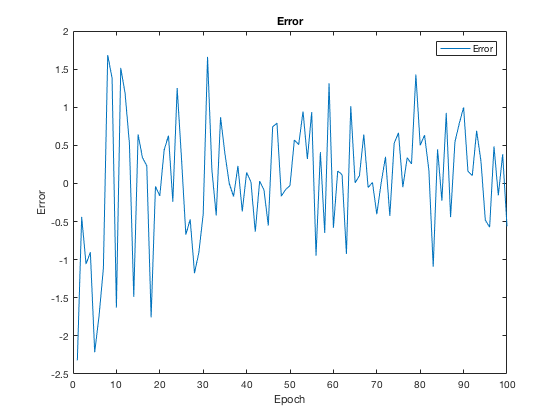
\includegraphics[width=0.4\textwidth]{error_time_01lr}
	\caption{Error for each training epoch (time-dependent), learning rate = 0.1\label{fig:err01time}}
\end{center}
\end{figure}
\end{centering}

\begin{centering}
\begin{figure}
\begin{center}
	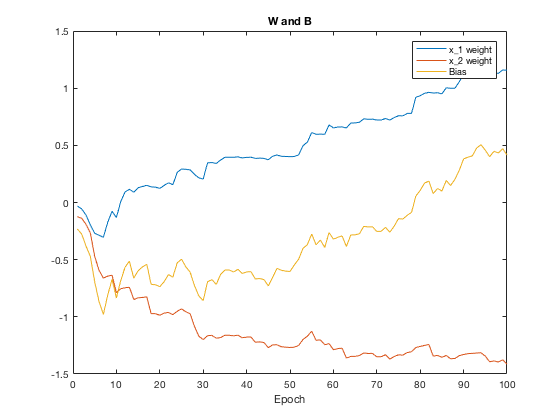
\includegraphics[width=0.4\textwidth]{weights_time_01lr}
	\caption{Weights for each training epoch (time-dependent), learning rate = 0.1\label{fig:wgt01time}}
\end{center}
\end{figure}
\end{centering}

\begin{centering}
\begin{figure}
\begin{center}
	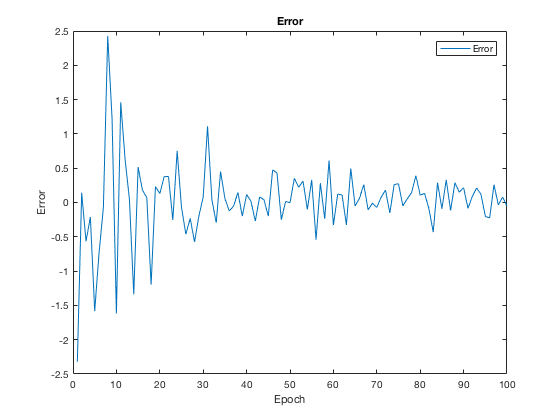
\includegraphics[width=0.4\textwidth]{error_time_03lr}
	\caption{Error for each training epoch (time-dependent), learning rate = 0.3\label{fig:err03time}}
\end{center}
\end{figure}
\end{centering}

\begin{centering}
\begin{figure}
\begin{center}
	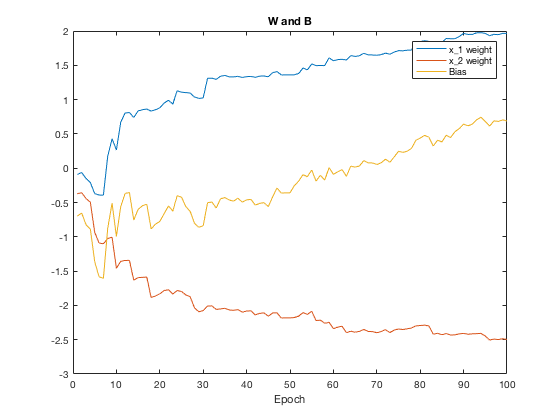
\includegraphics[width=0.4\textwidth]{weights_time_03lr}
	\caption{Weights for each training epoch (time-dependent), learning rate = 0.3\label{fig:wgt03time}}
\end{center}
\end{figure}
\end{centering}

With higher learning rates in place, the weights converged (see figs \ref{fig:err07time}, \ref{fig:wgt07time}, \ref{fig:err09time}, \ref{fig:wgt09time}), though not as closely as they had in the case of the time-independent function. The convergence time was similar in each case, around 30 epochs. It is theorized that after this time the network was sufficiently well trained to allow for only small corrections, thereby giving the appearance of a well-trained network.

\begin{centering}
\begin{figure}
\begin{center}
	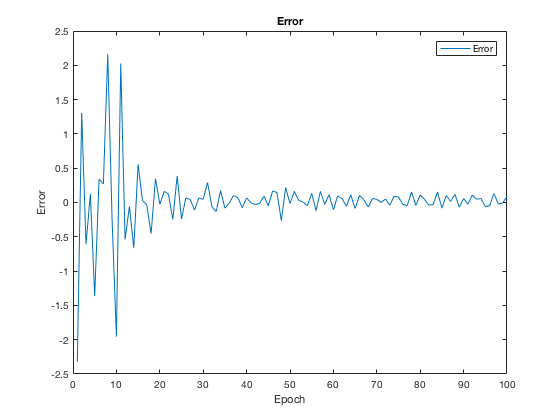
\includegraphics[width=0.4\textwidth]{error_time_07lr}
	\caption{Error for each training epoch (time-dependent), learning rate = 0.7\label{fig:err07time}}
\end{center}
\end{figure}
\end{centering}

\begin{centering}
\begin{figure}
\begin{center}
	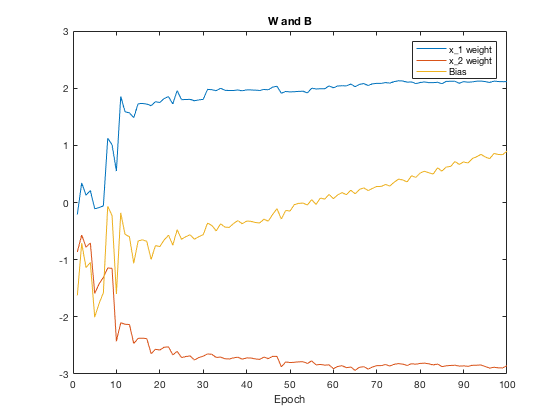
\includegraphics[width=0.4\textwidth]{weights_time_07lr}
	\caption{Weights for each training epoch (time-dependent), learning rate = 0.7\label{fig:wgt07time}}
\end{center}
\end{figure}
\end{centering}

\begin{centering}
\begin{figure}
\begin{center}
	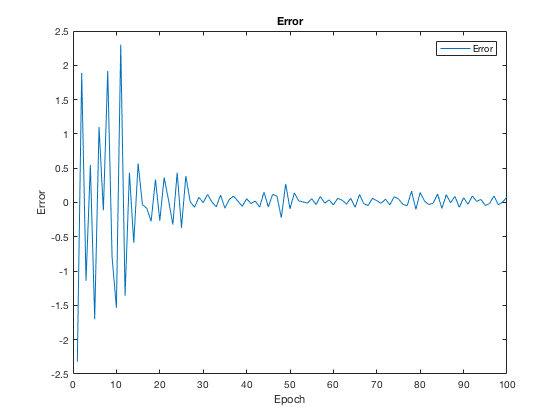
\includegraphics[width=0.4\textwidth]{error_time_09lr}
	\caption{Error for each training epoch (time-dependent), learning rate = 0.9\label{fig:err09time}}
\end{center}
\end{figure}
\end{centering}

\begin{centering}
\begin{figure}
\begin{center}
	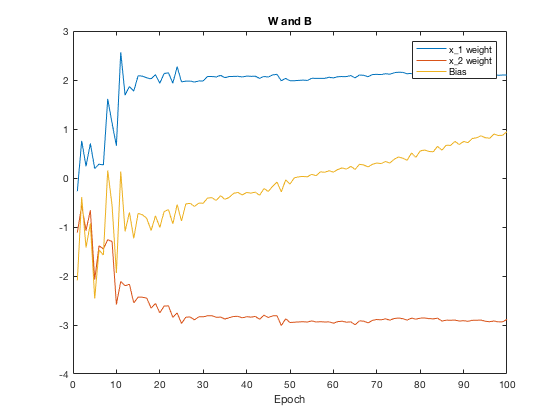
\includegraphics[width=0.4\textwidth]{weights_time_09lr}
	\caption{Weights for each training epoch (time-dependent), learning rate = 0.9\label{fig:wgt09time}}
\end{center}
\end{figure}
\end{centering}

\section{Conclusions}
An analysis of the impact of learning rates on the ability of a neural network to model a linear function was performed. For short training times, learning rates of 0.3 or less were insufficient to accurately model the function studied. Higher learning rates converged more quickly, and modeled the function well.

The network was less capable of modeling a time-dependent function. The change in the equation with each time step meant that the low learning rate networks suffered even more, and were not able to converge on the correct weights. Higher learning rates helped this problem, though the errors never fell to the levels observed in the time-independent problem.

\end{document}